% =====================================================================
% FORM-AC-01 - Análisis de caso: fallo real en un sistema distribuido
% Caso: Cloudflare, 19 centros de datos (21 de junio de 2022)
% Equipo: CGMZ
%
% REPARTO - todos trabajan en ESTE archivo, por turnos:
%   Sección 1 Descripción ...... P1 -> P2 -> P3 -> P4
%   Sección 2 Causas raíz ....... P1 -> P2 -> P3 -> P4 (y su rama del .drawio)
%   Sección 3 Impacto ........... P1 -> P2 -> P3 -> P4
%   Sección 4 Unidad 1 .......... P1 -> P2 -> P3 -> P4
%   Sección 5 Mitigación ........ P1 -> P2 -> P3 -> P4
%   Sección 6 Lecciones PFC ..... P1 -> P2 -> P3 -> P4
%   Tabla C8 .................... una fila por integrante
%
% =====================================================================
\documentclass[10pt,a4paper]{article}

% ---------- Idioma y tipografía ----------
\usepackage[utf8]{inputenc}
\usepackage[T1]{fontenc}
\usepackage[spanish,es-noshorthands]{babel}
\usepackage{newtxtext,newtxmath}
\usepackage{microtype}
\usepackage{csquotes}

% ---------- Página ----------
\usepackage[margin=2.2cm,headheight=14pt]{geometry}
\usepackage{array,tabularx,booktabs}
\usepackage{graphicx}
\usepackage{xcolor}
\usepackage{caption}
\usepackage{fancyhdr}
\usepackage[backend=biber,style=ieee,sorting=none]{biblatex}
\addbibresource{referencias.bib}
\usepackage{xurl}
\usepackage[hidelinks,breaklinks=true]{hyperref}
\urlstyle{same}

\graphicspath{{diagramas/}}
\captionsetup{font=small,labelfont=bf,skip=2pt}
\addto\captionsspanish{\renewcommand{\tablename}{Tabla}}

\setlength{\parindent}{0pt}
\setlength{\parskip}{3pt}
\setlength{\emergencystretch}{2em}
\renewcommand{\arraystretch}{1.15}
\setlength{\tabcolsep}{4pt}

% Marcador de texto faltante. Debe desaparecer en v2-final.
\newcommand{\pend}[1]{\textcolor{red}{\textbf{[PENDIENTE: #1]}}}

\pagestyle{fancy}
\fancyhf{}
\fancyhead[L]{\footnotesize FORM-AC-01}
\fancyhead[R]{\footnotesize Aplicaciones Distribuidas}
\fancyfoot[C]{\footnotesize Página \thepage}
\renewcommand{\headrulewidth}{0.4pt}

\begin{document}

% =====================================================================
% CARÁTULA (no cuenta para las 2 páginas) - la completa P1
% =====================================================================
\begin{titlepage}
\centering
{\scshape\large Universidad Técnica Estatal de Quevedo\par}
{\scshape Facultad de Ciencias de la Computación - Carrera de Software\par}
\vspace{1.2cm}
{\Large\bfseries Análisis de caso: fallo real en un sistema distribuido\par}
\vspace{0.3cm}
{\large FORM-AC-01 - Aplicaciones Distribuidas (ISR-701)\par}
\vspace{1.4cm}
{\large\bfseries Caso: Cloudflare, 19 centros de datos (21 de junio de 2022)\par}
\vspace{1.4cm}
\begin{tabular}{@{}ll@{}}
Equipo:      & CGMZ \\
Integrantes: & ZAMBRANO PARRAGA LUIS MARIO (P1) \\
             & MERA JUMBO ALLISON MICHELLE (P2) \\
             & CALDERON SALTOS JOSEPH ALEXANDER (P3) \\
             & GARCIA SANGOQUIZA ROGER STEVEN (P4) \\
Paralelo:    & A \\
Semestre:    & Séptimo \\
Fecha:       & 14 de noviembre de 2026 \\
Docente:     & Gleiston C. Guerrero-Ulloa, PhD \\
\end{tabular}
\vfill
{\footnotesize\url{https://github.com/Yukisan-uwo/FORM-AC-01-Analisis-de-Caso-Fallo-en-Sistema-Distribuido-Real.git}\par}
\end{titlepage}
\setcounter{page}{2}

% =====================================================================
% CONTENIDO EVALUABLE: máximo 2 páginas desde aquí
% =====================================================================

% ---------------------------------------------------------------------
% SECCIÓN 1 - DESCRIPCIÓN.
% ---------------------------------------------------------------------
\section{Descripción del incidente}
Cloudflare es una red de entrega de contenido y de seguridad que atiende tráfico en todo el mundo desde centros de datos distribuidos. Sus 19 ubicaciones más ocupadas ---en América, Europa y Asia--- usan la arquitectura Multi-Colo PoP (MCP), una red Clos con una capa de enrutamiento (spines) que permite habilitar y deshabilitar partes de la red interna sin cortar el tráfico. Para ser alcanzable, cada ubicación anuncia sus prefijos mediante BGP; si una política deja de anunciarlos, esas direcciones quedan inalcanzables. Eso ocurrió el 21 de junio de 2022: el incidente comenzó a las 06:27 UTC y el servicio se restableció a las 07:42 UTC \cite{cloudflare2022}.

\begin{center}
\captionof{table}{Línea de tiempo del incidente (todas las horas en UTC)}
\small
\begin{tabularx}{\linewidth}{@{}lX@{}}
\toprule
Hora (UTC) & Evento \\
\midrule
03:56 & Se despliega el cambio en la primera ubicación, de arquitectura antigua; ninguna ubicación resulta afectada \cite{cloudflare2022} \\
06:17 & Se despliega el cambio en las ubicaciones más ocupadas, pero todavía sin arquitectura MCP \cite{cloudflare2022} \\
06:27 & El despliegue llega a las ubicaciones con arquitectura MCP y el cambio se aplica en sus spines; las 19 ubicaciones quedan fuera de servicio y comienza el incidente \cite{cloudflare2022} \\
06:32 & Cloudflare declara internamente el incidente \cite{cloudflare2022} \\
06:51 & \pend{P3: primer cambio en un router para verificar la causa} \\
06:58 & \pend{P3: causa raíz entendida; empieza la reversión; vuelve el primer DC} \\
07:42 & \pend{P4: última reversión; los 19 DC están en línea (demora por reverts cruzados)} \\
08:00 & \pend{P4: cierre del incidente} \\
\bottomrule
\end{tabularx}
\end{center}

\pend{P4: duración total (75 min hasta restaurar el servicio y 93 min hasta el cierre) y lectura breve de la secuencia}

% ---------------------------------------------------------------------
% SECCIÓN 2 - CAUSAS RAÍZ
% ---------------------------------------------------------------------
\section{Causas raíz}
El incidente se explica en tres niveles: un detonante técnico, causas que amplificaron su efecto y defensas que debían contenerlo y no lo hicieron \cite{cloudflare2022}. La causa raíz pasa la prueba de que, sin ella, la caída no habría ocurrido: el orden de los términos de una política de anuncio.

\begin{center}
\IfFileExists{diagramas/causas.pdf}{%
  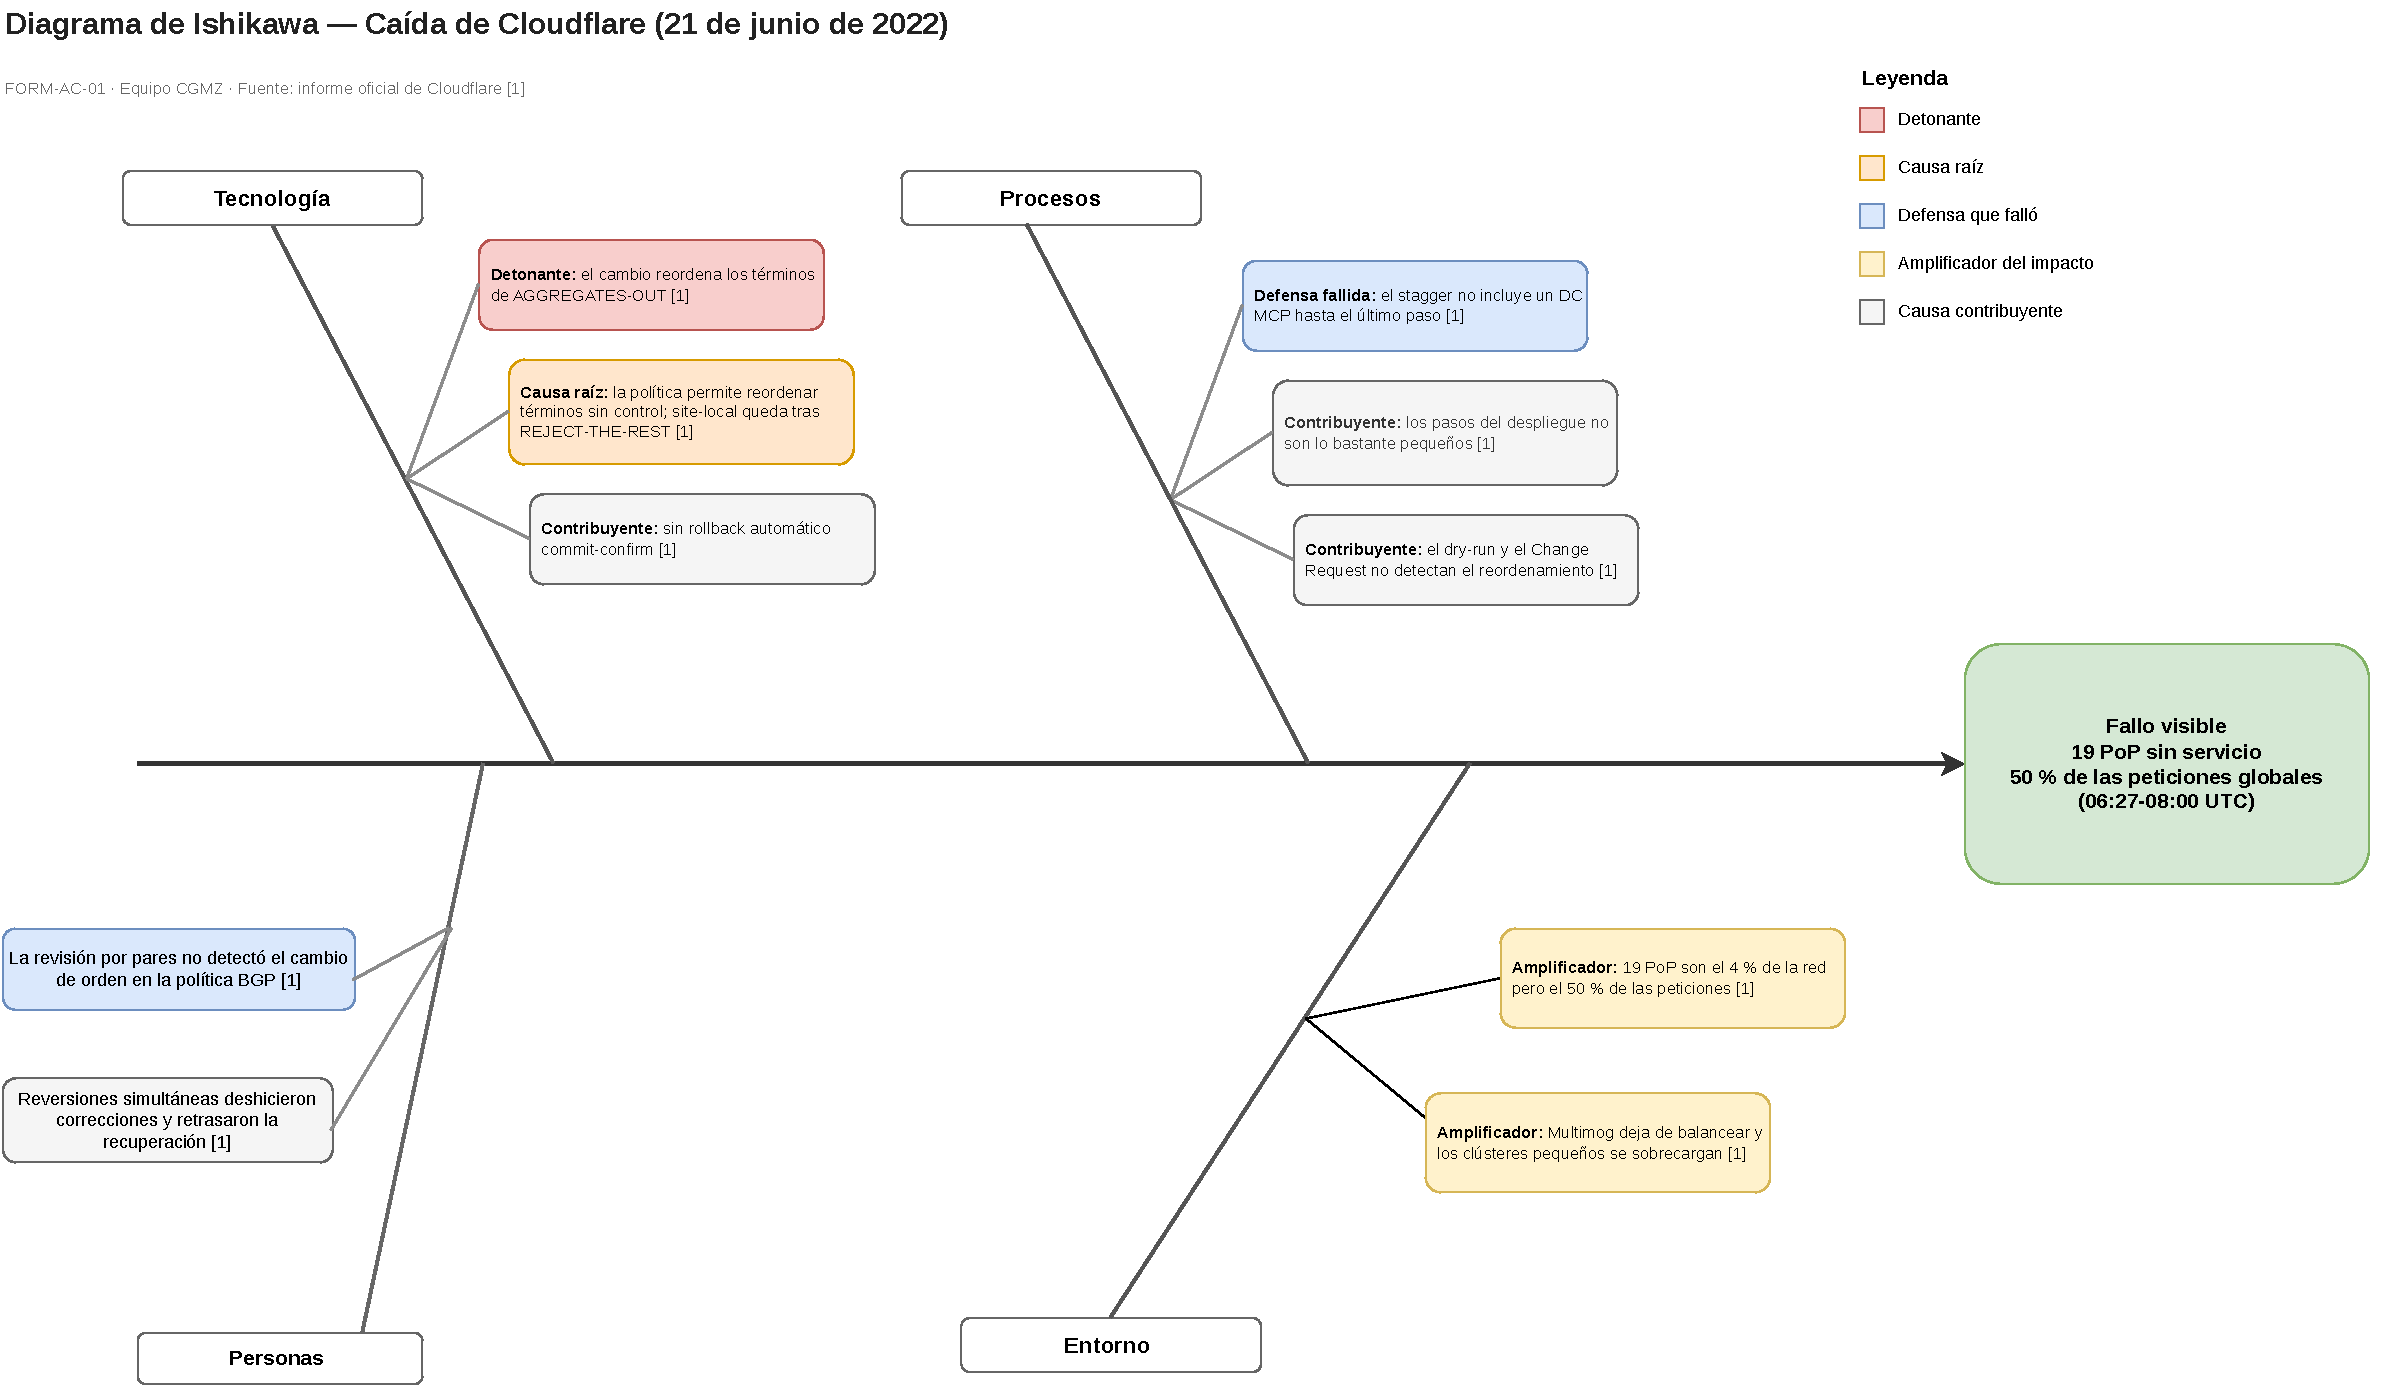
\includegraphics[width=0.92\linewidth]{diagramas/causas.pdf}%
}{%
  \fbox{\parbox[c][5cm][c]{0.85\linewidth}{\centering
  \pend{P2: exportar diagramas/causas.pdf desde causas.drawio}}}%
}
\captionof{figure}{Diagrama de Ishikawa del incidente. Elaboración propia en draw.io.}
\end{center}

\paragraph{Tecnología.}
El cambio buscaba estandarizar las \emph{communities} BGP asociadas a los prefijos \emph{site-local}, que permiten que los servidores de un MCP se comuniquen entre sí y alcancen los orígenes de los clientes. En los spines, el diff reordenó los términos de la política \texttt{AGGREGATES-OUT}: \texttt{4-ADV-SITE-LOCALS} y \texttt{6-ADV-SITE-LOCALS} pasaron al final, detrás de \texttt{REJECT-THE-REST}, un término que rechaza de forma explícita todo lo que le sigue. Desde ese momento Cloudflare dejó de anunciar los prefijos site-local y perdió el acceso directo a las ubicaciones afectadas y a los orígenes \cite{cloudflare2022}. El reordenamiento es el detonante; que la política pudiera reordenarse sin un control que lo impidiera es la causa raíz.

\paragraph{Procesos.}
El cambio contaba con un \emph{dry-run} y un despliegue escalonado (\emph{stagger}), pero ninguna de las dos defensas lo contuvo: el \emph{stagger} no incluía un centro de datos MCP hasta el último paso y sus pasos no eran lo bastante pequeños para detener el error antes de que alcanzara todos los spines \cite{cloudflare2022}. Ghosh et al. observan el mismo patrón: buena parte de los errores de configuración proviene de cambios recientes y podría detectarse con pruebas más rigurosas \cite{ghosh2022}.

\paragraph{Personas (P3).}
\pend{P3: la revisión por pares no vio el reordenamiento; los reverts cruzados alargaron la recuperación}

\paragraph{Entorno (P4).}
\pend{P4: 19 PoP = 4 \% de la red pero 50 \% del tráfico; Multimog dejó de balancear y sobrecargó los clusters pequeños}

% ---------------------------------------------------------------------
% SECCIÓN 3 - IMPACTO. ORDEN: P1 -> P2 -> P3 -> P4
% ---------------------------------------------------------------------
\section{Impacto cuantificado}
\begin{itemize}
  \item 19 centros de datos afectados, equivalentes al 4 \% de la red de Cloudflare \cite{cloudflare2022}.
  \item \pend{P2: 50 \% de las peticiones HTTP globales afectadas, con cita}
  \item \pend{P3: 75 min hasta la restauración total; 93 min hasta el cierre, con cita}
  \item \pend{P4: disponibilidad del mes: (43\,200 - 75)/43\,200 = 99,83 \%; el informe no reporta pérdida económica, de datos ni el SLA contractual}
\end{itemize}

% ---------------------------------------------------------------------
% SECCIÓN 4 - UNIDAD 1. ORDEN: P1 -> P2 -> P3 -> P4
% ---------------------------------------------------------------------
\section{Relación con la Unidad 1}
\paragraph{Transparencia (P1).}
Se rompió la transparencia de ubicación: el usuario no debía notar desde qué centro de datos lo atendían, pero el informe reconoce que, según su ubicación en el mundo, pudo quedar sin acceso a sitios y servicios que dependen de Cloudflare, mientras en otras regiones la red seguía operando con normalidad \cite{cloudflare2022}. De forma secundaria se rompió la transparencia de fallos: la caída fue visible y la recuperación exigió intervención manual de los ingenieros.

\paragraph{CAP (P2).}
\pend{P2: hubo partición de facto por el withdraw; no fue un trade-off C/A deliberado; CAP no explica la causa}

\paragraph{Tolerancia a fallos (P3).}
\pend{P3: malla Clos/MCP, Multimog y stagger; cuál no funcionó y por qué}

\paragraph{Modelo de fallo (P4).}
\pend{P4: fallo por omisión con caída efectiva; cierre del apartado}

% ---------------------------------------------------------------------
% SECCIÓN 5 - MITIGACIÓN. ORDEN: P1 -> P2 -> P3 -> P4
% P1 y P2: medidas inmediatas. P3 y P4: cambios permanentes.
% ---------------------------------------------------------------------
\section{Mitigación aplicada por la empresa}
\paragraph{Medidas inmediatas.}
Se revirtió el cambio defectuoso; a las 06:58 volvió a estar en línea el primer centro de datos \cite{cloudflare2022}.
\pend{P2: procedimientos de respaldo para recuperar el control de las ubicaciones}

\paragraph{Cambios permanentes.}
\pend{P3: proceso de cambio y despliegue específico para MCP}
\pend{P4: rediseño de la política y automatización (stagger + commit-confirm)}

\begin{center}
\captionof{table}{Cada medida contra la causa del diagrama que ataca}
\small
\begin{tabularx}{\linewidth}{@{}p{4.2cm}lX@{}}
\toprule
Medida & Tipo & Causa que ataca \\
\midrule
Reversión del cambio & Inmediata & Detonante: orden incorrecto de los términos \cite{cloudflare2022} \\
\pend{P2: fila 2} & Inmediata  & \pend{P2} \\
\pend{P3: fila 3} & Permanente & \pend{P3} \\
\pend{P4: fila 4} & Permanente & \pend{P4} \\
\bottomrule
\end{tabularx}
\end{center}

% ---------------------------------------------------------------------
% SECCIÓN 6 - LECCIONES PARA EL PFC. ORDEN: P1 -> P2 -> P3 -> P4
% Un riesgo por integrante (la guía pide al menos tres).
% ---------------------------------------------------------------------
\section{Lecciones aprendidas para el proyecto propio}
Los proyectos del equipo comparten con Cloudflare una dependencia de servicios centrales: una base de datos, un servicio de avisos y una configuración que se aplica a varios nodos. Los riesgos siguientes son los puntos donde un fallo pequeño podría escalar como en el caso analizado.

\begin{center}
\captionof{table}{Riesgos del PFC y medidas preventivas para TA-PFC-E1}
\scriptsize
\begin{tabularx}{\linewidth}{@{}p{2.3cm}XXp{3.1cm}X@{}}
\toprule
Riesgo (componente) & Escenario de fallo & Relación con el caso & Medida para TA-PFC-E1 & Cómo se verifica \\
\midrule
Base de datos y aviso de confirmación (SGRA) & La confirmación de un refuerzo y el aviso al estudiante pasan por un único servidor; si el proceso se interrumpe, el refuerzo queda asignado sin aviso o el reintento lo duplica & Un fallo en un componente compartido afecta a todos los usuarios a la vez, como en Cloudflare & Registrar asignación y aviso en una sola transacción, con reintentos idempotentes & Detener el aviso, crear un refuerzo y comprobar que se confirma una sola vez y se notifica al reactivar, sin duplicados \\
\pend{R2 P2} & \pend{} & \pend{} & \pend{} & \pend{} \\
\pend{R3 P3} & \pend{} & \pend{} & \pend{} & \pend{} \\
\pend{R4 P4} & \pend{} & \pend{} & \pend{} & \pend{} \\
\bottomrule
\end{tabularx}
\end{center}

% =====================================================================
% NO CUENTA PARA LAS 2 PÁGINAS
% =====================================================================

% ---------------------------------------------------------------------
% TABLA C8 - una fila por integrante, con una observación real de la
% revisión interna (no hay sesión de pares: el docente no la programó).
% ---------------------------------------------------------------------
\section*{Tabla de retroalimentación incorporada}
\begin{center}
\small
\begin{tabularx}{\linewidth}{@{}p{0.6cm}p{2.2cm}XX@{}}
\toprule
N. & Origen & Observación recibida & Cambio realizado o razón para no aplicarlo \\
\midrule
1 & Revisión interna (equipo) & La transparencia de fallos quedaba enunciada sin respaldo textual del informe. & Se añadió la cita al hecho de que la recuperación exigió intervención manual de los ingenieros; se ve en §4, párrafo Transparencia. \\
2 & \pend{quién observó} & \pend{P2} & \pend{} \\
3 & \pend{quién observó} & \pend{P3} & \pend{} \\
4 & \pend{quién observó} & \pend{P4} & \pend{} \\
\bottomrule
\end{tabularx}
\end{center}

{\footnotesize Nota: el docente no programó la sesión de exposición ni la evaluación entre pares; por eso las observaciones provienen de la revisión interna entre los cuatro integrantes. Las hojas de pares, de existir, están en \texttt{pares/}.}

% ---------------------------------------------------------------------
% DECLARACIÓN DE USO DE IA
% ---------------------------------------------------------------------
\section*{Declaración de uso de inteligencia artificial}
Herramienta: opencode (asistente de línea de comandos). Uso: ordenar la línea de tiempo. Verificación: cada cifra y cada cita se contrastó con el informe oficial, y cada DOI se resolvió en \url{https://doi.org} y se comparó con Crossref.

\printbibliography

\end{document}
